Nel Frontend è stato utilizzato il pattern architetturale Model-View-Presenter (MVP), design diffuso nelle WebApp, con lo scopo di separare le componenti di
visualizzazione dalla loro implementazione.
Il pattern si suddivide in tre elementi:
\begin{itemize}
    \item Model : elemento dove sono definiti i dati
    \item View : elemento per la visualizzazione dei dati
    \item Presenter : elemento mediatore che preleva i dati dal Model e li formatta per la View
\end{itemize}
Quando l'utente interagisce con l'applicazione, la parte di View è incaricata di visualizzare i dati 
e di notificare le azioni dell'utente, la parte del Presenter fa da tramite per le interazioni tra View e Model, prelevando i dati da quest'ultimo e visualizzandoli.
Il Model, per ottenere i dati, richiama una API (tramite metodo POST o GET) che si occuperà di interfacciarsi con
il Backend, il quale si occuperà di restituire i dati in caso di esito positivo.


\begin{figure}[!h]
    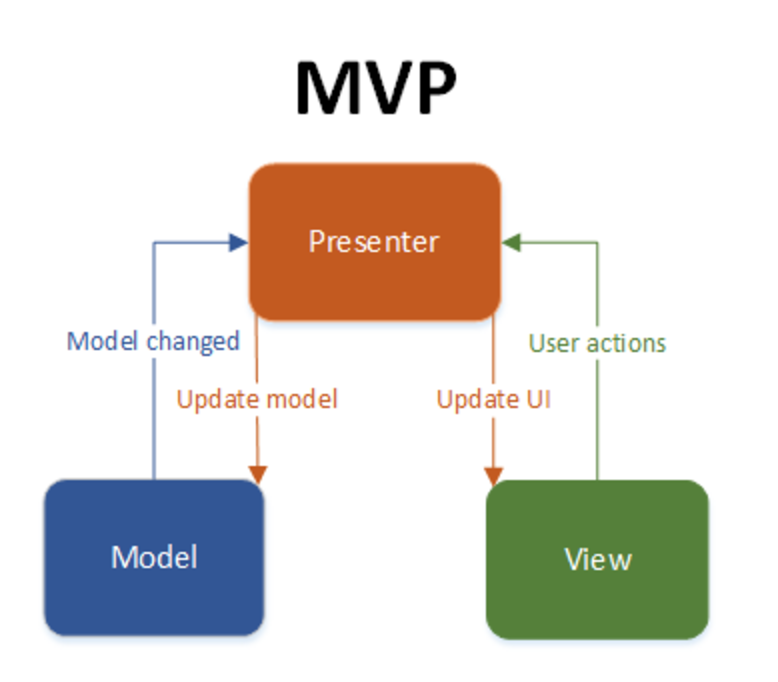
\includegraphics[width=16cm]{sezioni/images/mvp.png}
    \centering
    \caption{Schema pattern MVP}
\end{figure}

I punti di forza individuati in questo pattern sono che ogni classe Presenter possa gestire 
una classe View alla volta, quindi l'esistenza di una relazione uno a uno e questo permette di avere maggiore 
controllo sulle varie componenti, e la netta separazione presente tra Model e View. 
Quest'ultima risulta un punto chiave perchè permette di facilitare il testing relativo ai Presenter.

\subsection{Diagramma delle classi}
\begin{figure}[!h]
    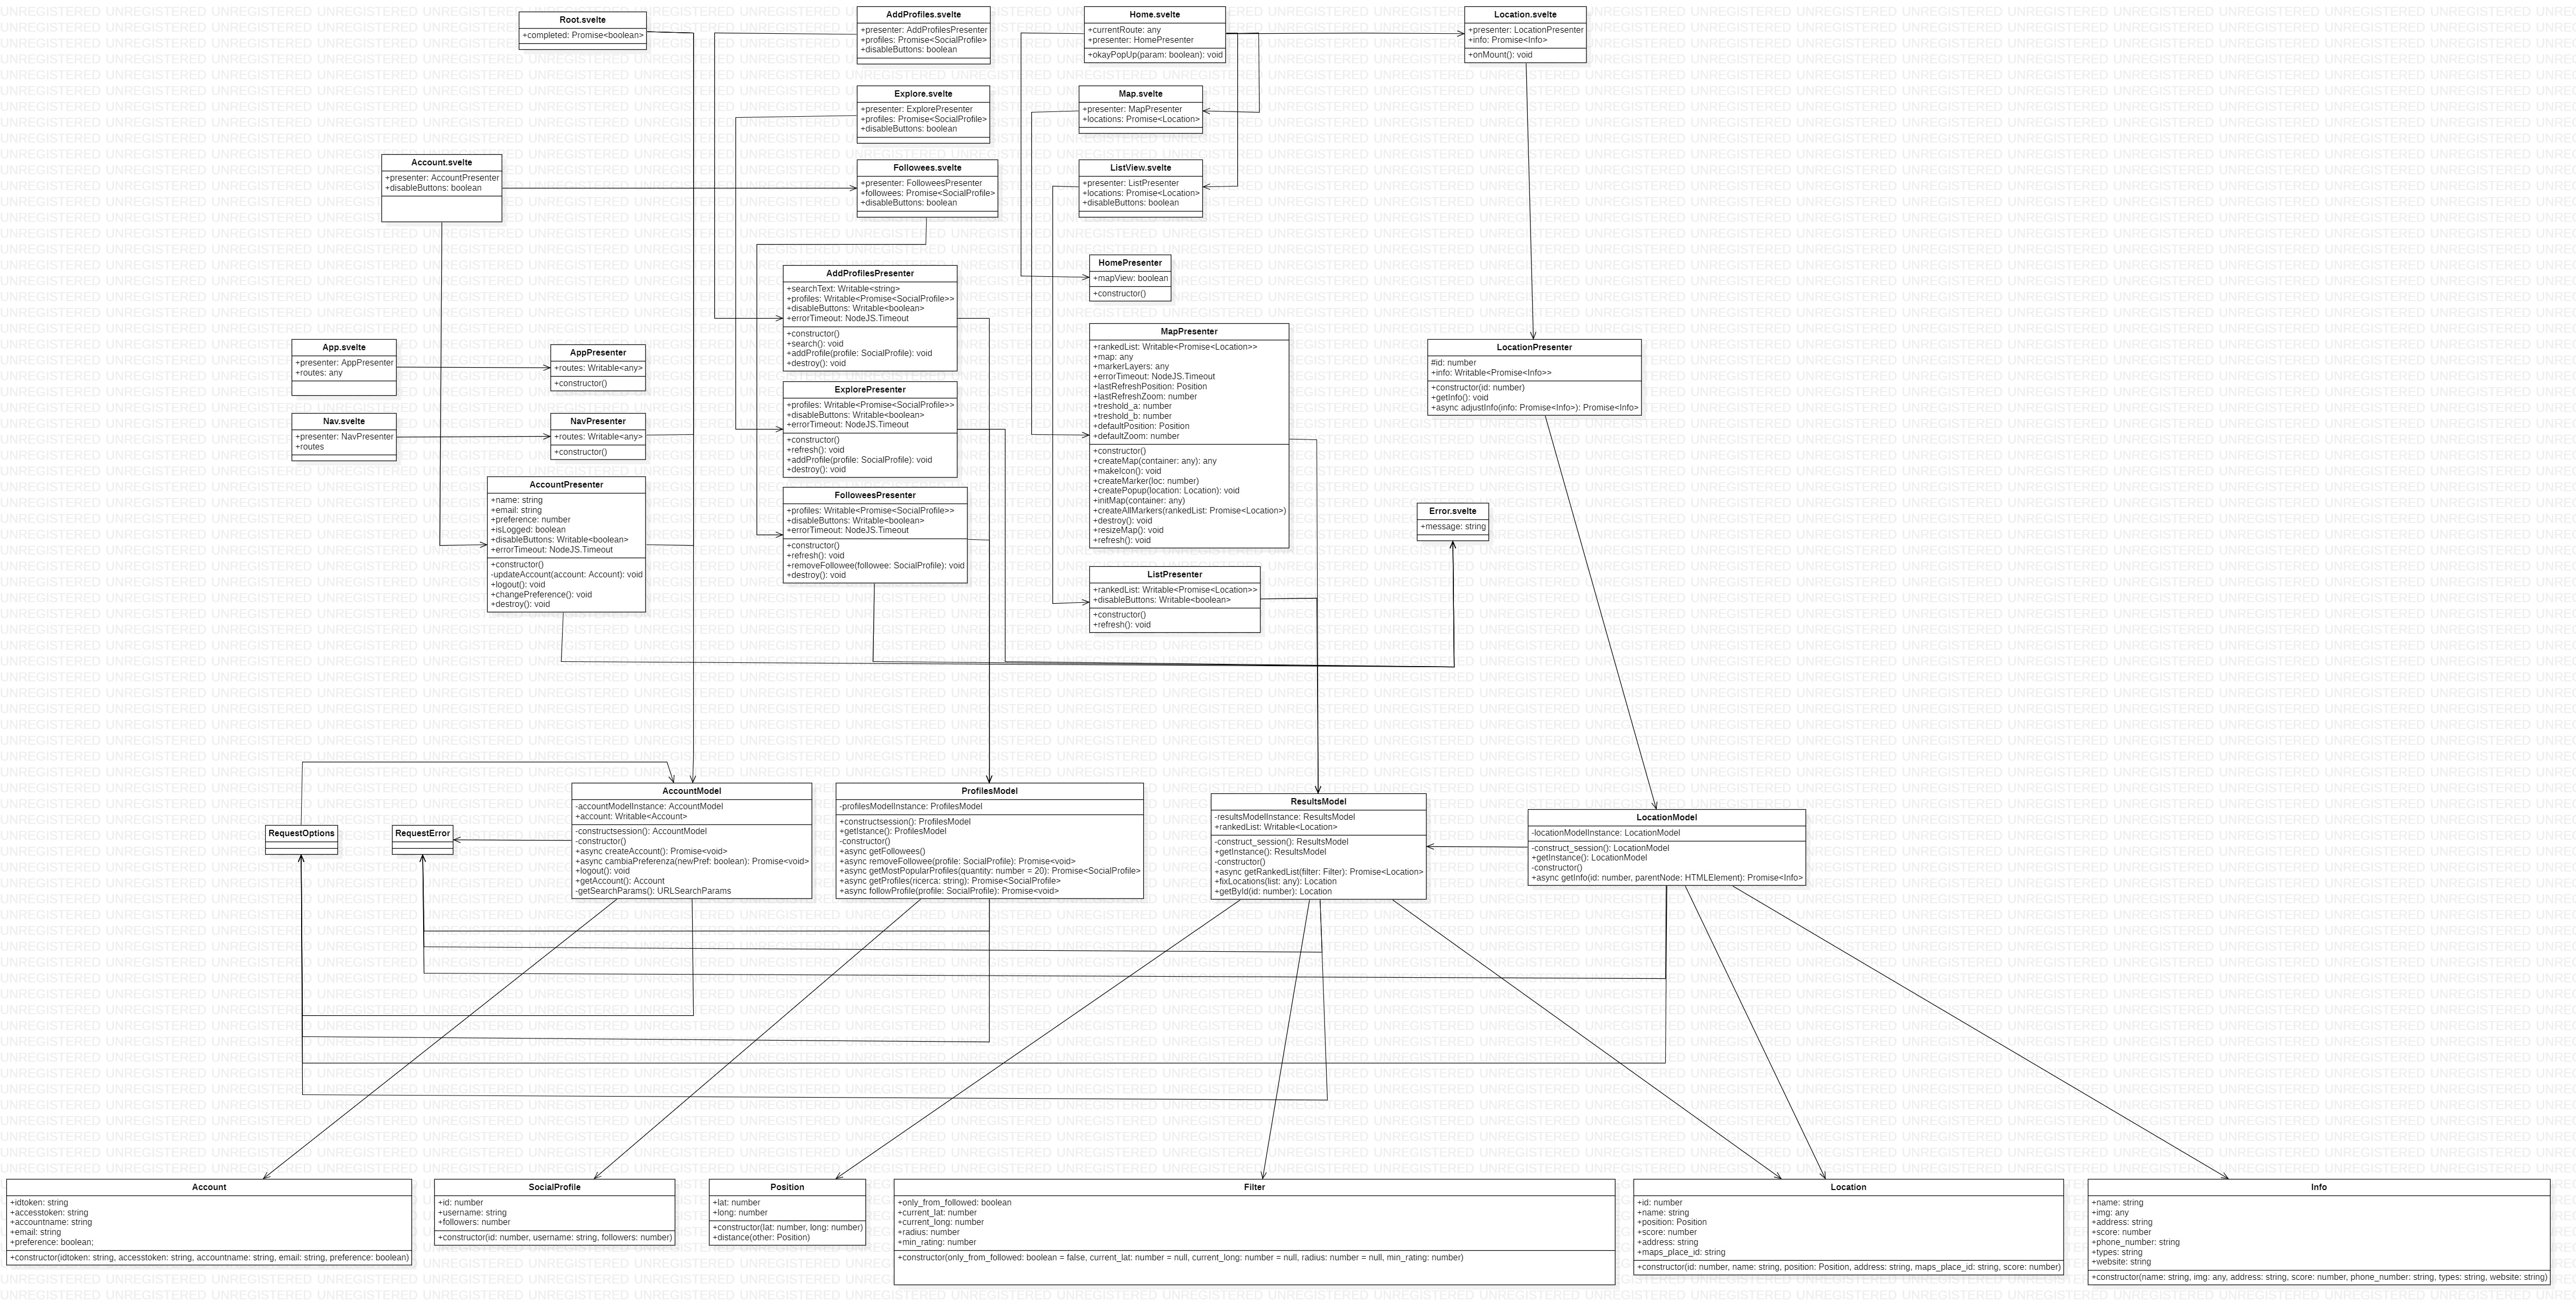
\includegraphics[width=16cm]{sezioni/images/Main.jpg}
    \centering
    \caption{Frontend - Diagramma delle classi}
\end{figure}

